\documentclass[1p]{elsarticle_modified}
%\bibliographystyle{elsarticle-num}

%\usepackage[colorlinks]{hyperref}
%\usepackage{abbrmath_seonhwa} %\Abb, \Ascr, \Acal ,\Abf, \Afrak
\usepackage{amsfonts}
\usepackage{amssymb}
\usepackage{amsmath}
\usepackage{amsthm}
\usepackage{scalefnt}
\usepackage{amsbsy}
\usepackage{kotex}
\usepackage{caption}
\usepackage{subfig}
\usepackage{color}
\usepackage{graphicx}
\usepackage{xcolor} %% white, black, red, green, blue, cyan, magenta, yellow
\usepackage{float}
\usepackage{setspace}
\usepackage{hyperref}

\usepackage{tikz}
\usetikzlibrary{arrows}

\usepackage{multirow}
\usepackage{array} % fixed length table
\usepackage{hhline}

%%%%%%%%%%%%%%%%%%%%%
\makeatletter
\renewcommand*\env@matrix[1][\arraystretch]{%
	\edef\arraystretch{#1}%
	\hskip -\arraycolsep
	\let\@ifnextchar\new@ifnextchar
	\array{*\c@MaxMatrixCols c}}
\makeatother %https://tex.stackexchange.com/questions/14071/how-can-i-increase-the-line-spacing-in-a-matrix
%%%%%%%%%%%%%%%

\usepackage[normalem]{ulem}

\newcommand{\msout}[1]{\ifmmode\text{\sout{\ensuremath{#1}}}\else\sout{#1}\fi}
%SOURCE: \msout is \stkout macro in https://tex.stackexchange.com/questions/20609/strikeout-in-math-mode

\newcommand{\cancel}[1]{
	\ifmmode
	{\color{red}\msout{#1}}
	\else
	{\color{red}\sout{#1}}
	\fi
}

\newcommand{\add}[1]{
	{\color{blue}\uwave{#1}}
}

\newcommand{\replace}[2]{
	\ifmmode
	{\color{red}\msout{#1}}{\color{blue}\uwave{#2}}
	\else
	{\color{red}\sout{#1}}{\color{blue}\uwave{#2}}
	\fi
}

\newcommand{\Sol}{\mathcal{S}} %segment
\newcommand{\D}{D} %diagram
\newcommand{\A}{\mathcal{A}} %arc


%%%%%%%%%%%%%%%%%%%%%%%%%%%%%5 test

\def\sl{\operatorname{\textup{SL}}(2,\Cbb)}
\def\psl{\operatorname{\textup{PSL}}(2,\Cbb)}
\def\quan{\mkern 1mu \triangleright \mkern 1mu}

\theoremstyle{definition}
\newtheorem{thm}{Theorem}[section]
\newtheorem{prop}[thm]{Proposition}
\newtheorem{lem}[thm]{Lemma}
\newtheorem{ques}[thm]{Question}
\newtheorem{cor}[thm]{Corollary}
\newtheorem{defn}[thm]{Definition}
\newtheorem{exam}[thm]{Example}
\newtheorem{rmk}[thm]{Remark}
\newtheorem{alg}[thm]{Algorithm}

\newcommand{\I}{\sqrt{-1}}
\begin{document}

%\begin{frontmatter}
%
%\title{Boundary parabolic representations of knots up to 8 crossings}
%
%%% Group authors per affiliation:
%\author{Yunhi Cho} 
%\address{Department of Mathematics, University of Seoul, Seoul, Korea}
%\ead{yhcho@uos.ac.kr}
%
%
%\author{Seonhwa Kim} %\fnref{s_kim}}
%\address{Center for Geometry and Physics, Institute for Basic Science, Pohang, 37673, Korea}
%\ead{ryeona17@ibs.re.kr}
%
%\author{Hyuk Kim}
%\address{Department of Mathematical Sciences, Seoul National University, Seoul 08826, Korea}
%\ead{hyukkim@snu.ac.kr}
%
%\author{Seokbeom Yoon}
%\address{Department of Mathematical Sciences, Seoul National University, Seoul, 08826,  Korea}
%\ead{sbyoon15@snu.ac.kr}
%
%\begin{abstract}
%We find all boundary parabolic representation of knots up to 8 crossings.
%
%\end{abstract}
%\begin{keyword}
%    \MSC[2010] 57M25 
%\end{keyword}
%
%\end{frontmatter}

%\linenumbers
%\tableofcontents
%
\newcommand\colored[1]{\textcolor{white}{\rule[-0.35ex]{0.8em}{1.4ex}}\kern-0.8em\color{red} #1}%
%\newcommand\colored[1]{\textcolor{white}{ #1}\kern-2.17ex	\textcolor{white}{ #1}\kern-1.81ex	\textcolor{white}{ #1}\kern-2.15ex\color{red}#1	}

{\Large $\underline{12a_{0552}~(K12a_{0552})}$}

\setlength{\tabcolsep}{10pt}
\renewcommand{\arraystretch}{1.6}
\vspace{1cm}\begin{tabular}{m{100pt}>{\centering\arraybackslash}m{274pt}}
\multirow{5}{120pt}{
	\centering
	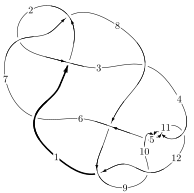
\includegraphics[width=112pt]{../../../GIT/diagram.site/Diagrams/png/1353_12a_0552.png}\\
\ \ \ A knot diagram\footnotemark}&
\allowdisplaybreaks
\textbf{Linearized knot diagam} \\
\cline{2-2}
 &
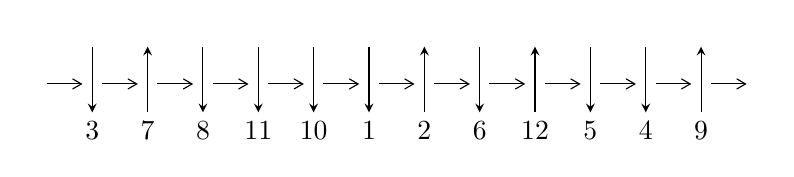
\begin{tikzpicture}[x=20pt, y=17pt]
	% nodes
	\node (C0) at (0, 0) {};
	\node (C1) at (1, 0) {};
	\node (C1U) at (1, +1) {};
	\node (C1D) at (1, -1) {3};

	\node (C2) at (2, 0) {};
	\node (C2U) at (2, +1) {};
	\node (C2D) at (2, -1) {7};

	\node (C3) at (3, 0) {};
	\node (C3U) at (3, +1) {};
	\node (C3D) at (3, -1) {8};

	\node (C4) at (4, 0) {};
	\node (C4U) at (4, +1) {};
	\node (C4D) at (4, -1) {11};

	\node (C5) at (5, 0) {};
	\node (C5U) at (5, +1) {};
	\node (C5D) at (5, -1) {10};

	\node (C6) at (6, 0) {};
	\node (C6U) at (6, +1) {};
	\node (C6D) at (6, -1) {1};

	\node (C7) at (7, 0) {};
	\node (C7U) at (7, +1) {};
	\node (C7D) at (7, -1) {2};

	\node (C8) at (8, 0) {};
	\node (C8U) at (8, +1) {};
	\node (C8D) at (8, -1) {6};

	\node (C9) at (9, 0) {};
	\node (C9U) at (9, +1) {};
	\node (C9D) at (9, -1) {12};

	\node (C10) at (10, 0) {};
	\node (C10U) at (10, +1) {};
	\node (C10D) at (10, -1) {5};

	\node (C11) at (11, 0) {};
	\node (C11U) at (11, +1) {};
	\node (C11D) at (11, -1) {4};

	\node (C12) at (12, 0) {};
	\node (C12U) at (12, +1) {};
	\node (C12D) at (12, -1) {9};
	\node (C13) at (13, 0) {};

	% arrows
	\draw[->,>={angle 60}]
	(C0) edge (C1) (C1) edge (C2) (C2) edge (C3) (C3) edge (C4) (C4) edge (C5) (C5) edge (C6) (C6) edge (C7) (C7) edge (C8) (C8) edge (C9) (C9) edge (C10) (C10) edge (C11) (C11) edge (C12) (C12) edge (C13) ;	\draw[->,>=stealth]
	(C1U) edge (C1D) (C2D) edge (C2U) (C3U) edge (C3D) (C4U) edge (C4D) (C5U) edge (C5D) (C6U) edge (C6D) (C7D) edge (C7U) (C8U) edge (C8D) (C9D) edge (C9U) (C10U) edge (C10D) (C11U) edge (C11D) (C12D) edge (C12U) ;
	\end{tikzpicture} \\
\hhline{~~} \\& 
\textbf{Solving Sequence} \\ \cline{2-2} 
 &
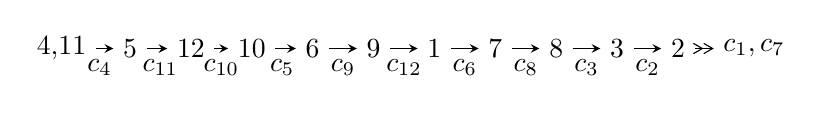
\begin{tikzpicture}[x=22pt, y=7pt]
	% node
	\node (A0) at (-1/8, 0) {4,11};
	\node (A1) at (1, 0) {5};
	\node (A2) at (2, 0) {12};
	\node (A3) at (3, 0) {10};
	\node (A4) at (4, 0) {6};
	\node (A5) at (5, 0) {9};
	\node (A6) at (6, 0) {1};
	\node (A7) at (7, 0) {7};
	\node (A8) at (8, 0) {8};
	\node (A9) at (9, 0) {3};
	\node (A10) at (10, 0) {2};
	\node (C1) at (1/2, -1) {$c_{4}$};
	\node (C2) at (3/2, -1) {$c_{11}$};
	\node (C3) at (5/2, -1) {$c_{10}$};
	\node (C4) at (7/2, -1) {$c_{5}$};
	\node (C5) at (9/2, -1) {$c_{9}$};
	\node (C6) at (11/2, -1) {$c_{12}$};
	\node (C7) at (13/2, -1) {$c_{6}$};
	\node (C8) at (15/2, -1) {$c_{8}$};
	\node (C9) at (17/2, -1) {$c_{3}$};
	\node (C10) at (19/2, -1) {$c_{2}$};
	\node (A11) at (45/4, 0) {$c_{1},c_{7}$};

	% edge
	\draw[->,>=stealth]	
	(A0) edge (A1) (A1) edge (A2) (A2) edge (A3) (A3) edge (A4) (A4) edge (A5) (A5) edge (A6) (A6) edge (A7) (A7) edge (A8) (A8) edge (A9) (A9) edge (A10) ;
	\draw[->>,>={angle 60}]	
	(A10) edge (A11);
\end{tikzpicture} \\ 

\end{tabular} \\

\footnotetext{
The image of knot diagram is generated by the software ``\textbf{Draw programme}" developed by Andrew Bartholomew(\url{http://www.layer8.co.uk/maths/draw/index.htm\#Running-draw}), where we modified some parts for our purpose(\url{https://github.com/CATsTAILs/LinksPainter}).
}\phantom \\ \newline 
\centering \textbf{Ideals for irreducible components\footnotemark of $X_{\text{par}}$} 
 
\begin{align*}
I^u_{1}&=\langle 
u^{65}+u^{64}+\cdots+3 u+1\rangle \\
\\
\end{align*}
\raggedright * 1 irreducible components of $\dim_{\mathbb{C}}=0$, with total 65 representations.\\
\footnotetext{All coefficients of polynomials are rational numbers. But the coefficients are sometimes approximated in decimal forms when there is not enough margin.}
\newpage
\renewcommand{\arraystretch}{1}
\centering \section*{I. $I^u_{1}= \langle u^{65}+u^{64}+\cdots+3 u+1 \rangle$}
\flushleft \textbf{(i) Arc colorings}\\
\begin{tabular}{m{7pt} m{180pt} m{7pt} m{180pt} }
\flushright $a_{4}=$&$\begin{pmatrix}1\\0\end{pmatrix}$ \\
\flushright $a_{11}=$&$\begin{pmatrix}0\\u\end{pmatrix}$ \\
\flushright $a_{5}=$&$\begin{pmatrix}1\\u^2\end{pmatrix}$ \\
\flushright $a_{12}=$&$\begin{pmatrix}- u\\u\end{pmatrix}$ \\
\flushright $a_{10}=$&$\begin{pmatrix}u\\u^3+u\end{pmatrix}$ \\
\flushright $a_{6}=$&$\begin{pmatrix}u^2+1\\u^4+2 u^2\end{pmatrix}$ \\
\flushright $a_{9}=$&$\begin{pmatrix}- u^5-2 u^3+u\\u^5+3 u^3+u\end{pmatrix}$ \\
\flushright $a_{1}=$&$\begin{pmatrix}- u^9-4 u^7-3 u^5+2 u^3- u\\u^9+5 u^7+7 u^5+2 u^3+u\end{pmatrix}$ \\
\flushright $a_{7}=$&$\begin{pmatrix}- u^{22}-11 u^{20}+\cdots-3 u^4+1\\u^{22}+12 u^{20}+\cdots+8 u^4+3 u^2\end{pmatrix}$ \\
\flushright $a_{8}=$&$\begin{pmatrix}u^{11}+6 u^9+12 u^7+8 u^5+u^3+2 u\\u^{13}+7 u^{11}+17 u^9+16 u^7+6 u^5+5 u^3+u\end{pmatrix}$ \\
\flushright $a_{3}=$&$\begin{pmatrix}- u^{24}-13 u^{22}+\cdots-2 u^2+1\\- u^{26}-14 u^{24}+\cdots-10 u^4- u^2\end{pmatrix}$ \\
\flushright $a_{2}=$&$\begin{pmatrix}- u^{59}-32 u^{57}+\cdots+5 u^3-2 u\\- u^{61}-33 u^{59}+\cdots+3 u^3+u\end{pmatrix}$\\&\end{tabular}
\flushleft \textbf{(ii) Obstruction class $= -1$}\\~\\
\flushleft \textbf{(iii) Cusp Shapes $= -4 u^{64}-4 u^{63}+\cdots-24 u-10$}\\~\\
\newpage\renewcommand{\arraystretch}{1}
\flushleft \textbf{(iv) u-Polynomials at the component}\newline \\
\begin{tabular}{m{50pt}|m{274pt}}
Crossings & \hspace{64pt}u-Polynomials at each crossing \\
\hline $$\begin{aligned}c_{1}\end{aligned}$$&$\begin{aligned}
&u^{65}+35 u^{64}+\cdots-3 u-1
\end{aligned}$\\
\hline $$\begin{aligned}c_{2},c_{7}\end{aligned}$$&$\begin{aligned}
&u^{65}+u^{64}+\cdots+u+1
\end{aligned}$\\
\hline $$\begin{aligned}c_{3},c_{6}\end{aligned}$$&$\begin{aligned}
&u^{65}- u^{64}+\cdots+u+1
\end{aligned}$\\
\hline $$\begin{aligned}c_{4},c_{5},c_{10}\\c_{11}\end{aligned}$$&$\begin{aligned}
&u^{65}+u^{64}+\cdots+3 u+1
\end{aligned}$\\
\hline $$\begin{aligned}c_{8}\end{aligned}$$&$\begin{aligned}
&u^{65}-9 u^{64}+\cdots-871 u+109
\end{aligned}$\\
\hline $$\begin{aligned}c_{9},c_{12}\end{aligned}$$&$\begin{aligned}
&u^{65}+11 u^{64}+\cdots+1417 u+187
\end{aligned}$\\
\hline
\end{tabular}\\~\\
\newpage\renewcommand{\arraystretch}{1}
\flushleft \textbf{(v) Riley Polynomials at the component}\newline \\
\begin{tabular}{m{50pt}|m{274pt}}
Crossings & \hspace{64pt}Riley Polynomials at each crossing \\
\hline $$\begin{aligned}c_{1}\end{aligned}$$&$\begin{aligned}
&y^{65}-9 y^{64}+\cdots+y-1
\end{aligned}$\\
\hline $$\begin{aligned}c_{2},c_{7}\end{aligned}$$&$\begin{aligned}
&y^{65}+35 y^{64}+\cdots-3 y-1
\end{aligned}$\\
\hline $$\begin{aligned}c_{3},c_{6}\end{aligned}$$&$\begin{aligned}
&y^{65}-53 y^{64}+\cdots-99 y-1
\end{aligned}$\\
\hline $$\begin{aligned}c_{4},c_{5},c_{10}\\c_{11}\end{aligned}$$&$\begin{aligned}
&y^{65}+71 y^{64}+\cdots-3 y-1
\end{aligned}$\\
\hline $$\begin{aligned}c_{8}\end{aligned}$$&$\begin{aligned}
&y^{65}-13 y^{64}+\cdots+40113 y-11881
\end{aligned}$\\
\hline $$\begin{aligned}c_{9},c_{12}\end{aligned}$$&$\begin{aligned}
&y^{65}+43 y^{64}+\cdots-640031 y-34969
\end{aligned}$\\
\hline
\end{tabular}\\~\\
\newpage\flushleft \textbf{(vi) Complex Volumes and Cusp Shapes}
$$\begin{array}{c|c|c}  
\text{Solutions to }I^u_{1}& \I (\text{vol} + \sqrt{-1}CS) & \text{Cusp shape}\\
 \hline 
\begin{aligned}
u &= -0.595719 + 0.578948 I\end{aligned}
 & -7.70647 + 11.34340 I & -8.26251 - 9.40428 I \\ \hline\begin{aligned}
u &= -0.595719 - 0.578948 I\end{aligned}
 & -7.70647 - 11.34340 I & -8.26251 + 9.40428 I \\ \hline\begin{aligned}
u &= -0.599254 + 0.561085 I\end{aligned}
 & -8.54295 + 2.41798 I & -9.80276 - 3.05774 I \\ \hline\begin{aligned}
u &= -0.599254 - 0.561085 I\end{aligned}
 & -8.54295 - 2.41798 I & -9.80276 + 3.05774 I \\ \hline\begin{aligned}
u &= \phantom{-}0.589572 + 0.570914 I\end{aligned}
 & -4.51819 - 6.51331 I & -5.31750 + 6.37538 I \\ \hline\begin{aligned}
u &= \phantom{-}0.589572 - 0.570914 I\end{aligned}
 & -4.51819 + 6.51331 I & -5.31750 - 6.37538 I \\ \hline\begin{aligned}
u &= \phantom{-}0.538749 + 0.569567 I\end{aligned}
 & -0.93086 - 6.41545 I & -3.67996 + 9.86351 I \\ \hline\begin{aligned}
u &= \phantom{-}0.538749 - 0.569567 I\end{aligned}
 & -0.93086 + 6.41545 I & -3.67996 - 9.86351 I \\ \hline\begin{aligned}
u &= \phantom{-}0.220912 + 0.733421 I\end{aligned}
 & -2.38478 - 6.60693 I & -2.78190 + 7.82097 I \\ \hline\begin{aligned}
u &= \phantom{-}0.220912 - 0.733421 I\end{aligned}
 & -2.38478 + 6.60693 I & -2.78190 - 7.82097 I \\ \hline\begin{aligned}
u &= \phantom{-}0.569041 + 0.489543 I\end{aligned}
 & -4.59319 - 1.95369 I & -11.39399 + 3.79158 I \\ \hline\begin{aligned}
u &= \phantom{-}0.569041 - 0.489543 I\end{aligned}
 & -4.59319 + 1.95369 I & -11.39399 - 3.79158 I \\ \hline\begin{aligned}
u &= -0.621187 + 0.418285 I\end{aligned}
 & -8.96370 + 1.72981 I & -11.03048 - 3.35966 I \\ \hline\begin{aligned}
u &= -0.621187 - 0.418285 I\end{aligned}
 & -8.96370 - 1.72981 I & -11.03048 + 3.35966 I \\ \hline\begin{aligned}
u &= -0.505578 + 0.547288 I\end{aligned}
 & -0.07972 + 2.16929 I & -1.40597 - 3.65142 I \\ \hline\begin{aligned}
u &= -0.505578 - 0.547288 I\end{aligned}
 & -0.07972 - 2.16929 I & -1.40597 + 3.65142 I \\ \hline\begin{aligned}
u &= -0.624357 + 0.395701 I\end{aligned}
 & -8.24591 - 7.19806 I & -9.88810 + 3.21124 I \\ \hline\begin{aligned}
u &= -0.624357 - 0.395701 I\end{aligned}
 & -8.24591 + 7.19806 I & -9.88810 - 3.21124 I \\ \hline\begin{aligned}
u &= \phantom{-}0.613226 + 0.403101 I\end{aligned}
 & -5.01179 + 2.41777 I & -6.90071 - 0.01179 I \\ \hline\begin{aligned}
u &= \phantom{-}0.613226 - 0.403101 I\end{aligned}
 & -5.01179 - 2.41777 I & -6.90071 + 0.01179 I \\ \hline\begin{aligned}
u &= \phantom{-}0.274381 + 0.668482 I\end{aligned}
 & -2.83652 + 1.62881 I & -4.05285 + 1.38314 I \\ \hline\begin{aligned}
u &= \phantom{-}0.274381 - 0.668482 I\end{aligned}
 & -2.83652 - 1.62881 I & -4.05285 - 1.38314 I \\ \hline\begin{aligned}
u &= -0.043462 + 0.719036 I\end{aligned}
 & \phantom{-}2.69348 + 2.02135 I & \phantom{-}4.11374 - 4.67175 I \\ \hline\begin{aligned}
u &= -0.043462 - 0.719036 I\end{aligned}
 & \phantom{-}2.69348 - 2.02135 I & \phantom{-}4.11374 + 4.67175 I \\ \hline\begin{aligned}
u &= -0.195350 + 0.687690 I\end{aligned}
 & \phantom{-}0.60698 + 2.16613 I & \phantom{-}0.97582 - 4.91748 I \\ \hline\begin{aligned}
u &= -0.195350 - 0.687690 I\end{aligned}
 & \phantom{-}0.60698 - 2.16613 I & \phantom{-}0.97582 + 4.91748 I \\ \hline\begin{aligned}
u &= \phantom{-}0.537336 + 0.377380 I\end{aligned}
 & -1.48399 + 2.68474 I & -5.93567 - 3.09855 I \\ \hline\begin{aligned}
u &= \phantom{-}0.537336 - 0.377380 I\end{aligned}
 & -1.48399 - 2.68474 I & -5.93567 + 3.09855 I \\ \hline\begin{aligned}
u &= -0.463936 + 0.448567 I\end{aligned}
 & -0.422225 + 1.251880 I & -2.42688 - 4.39107 I \\ \hline\begin{aligned}
u &= -0.463936 - 0.448567 I\end{aligned}
 & -0.422225 - 1.251880 I & -2.42688 + 4.39107 I\\
 \hline 
 \end{array}$$\newpage$$\begin{array}{c|c|c}  
\text{Solutions to }I^u_{1}& \I (\text{vol} + \sqrt{-1}CS) & \text{Cusp shape}\\
 \hline 
\begin{aligned}
u &= -0.15190 + 1.44967 I\end{aligned}
 & -2.33616 - 4.48271 I & \phantom{-0.000000 } 0 \\ \hline\begin{aligned}
u &= -0.15190 - 1.44967 I\end{aligned}
 & -2.33616 + 4.48271 I & \phantom{-0.000000 } 0 \\ \hline\begin{aligned}
u &= \phantom{-}0.14927 + 1.46063 I\end{aligned}
 & \phantom{-}0.981805 - 0.236082 I & \phantom{-0.000000 } 0 \\ \hline\begin{aligned}
u &= \phantom{-}0.14927 - 1.46063 I\end{aligned}
 & \phantom{-}0.981805 + 0.236082 I & \phantom{-0.000000 } 0 \\ \hline\begin{aligned}
u &= -0.16115 + 1.46529 I\end{aligned}
 & -2.88598 + 4.47628 I & \phantom{-0.000000 } 0 \\ \hline\begin{aligned}
u &= -0.16115 - 1.46529 I\end{aligned}
 & -2.88598 - 4.47628 I & \phantom{-0.000000 } 0 \\ \hline\begin{aligned}
u &= \phantom{-}0.09486 + 1.50450 I\end{aligned}
 & \phantom{-}4.62328 + 0.70657 I & \phantom{-0.000000 } 0 \\ \hline\begin{aligned}
u &= \phantom{-}0.09486 - 1.50450 I\end{aligned}
 & \phantom{-}4.62328 - 0.70657 I & \phantom{-0.000000 } 0 \\ \hline\begin{aligned}
u &= \phantom{-}0.486503 + 0.034595 I\end{aligned}
 & -4.82132 - 4.20427 I & -10.67761 + 3.89462 I \\ \hline\begin{aligned}
u &= \phantom{-}0.486503 - 0.034595 I\end{aligned}
 & -4.82132 + 4.20427 I & -10.67761 - 3.89462 I \\ \hline\begin{aligned}
u &= \phantom{-}0.15753 + 1.51877 I\end{aligned}
 & \phantom{-}2.03909 - 4.52101 I & \phantom{-0.000000 } 0 \\ \hline\begin{aligned}
u &= \phantom{-}0.15753 - 1.51877 I\end{aligned}
 & \phantom{-}2.03909 + 4.52101 I & \phantom{-0.000000 } 0 \\ \hline\begin{aligned}
u &= -0.12554 + 1.53196 I\end{aligned}
 & \phantom{-}6.27220 + 3.29095 I & \phantom{-0.000000 } 0 \\ \hline\begin{aligned}
u &= -0.12554 - 1.53196 I\end{aligned}
 & \phantom{-}6.27220 - 3.29095 I & \phantom{-0.000000 } 0 \\ \hline\begin{aligned}
u &= -0.14729 + 1.54850 I\end{aligned}
 & \phantom{-}6.93976 + 4.52566 I & \phantom{-0.000000 } 0 \\ \hline\begin{aligned}
u &= -0.14729 - 1.54850 I\end{aligned}
 & \phantom{-}6.93976 - 4.52566 I & \phantom{-0.000000 } 0 \\ \hline\begin{aligned}
u &= -0.18149 + 1.54544 I\end{aligned}
 & -1.55418 + 5.25395 I & \phantom{-0.000000 } 0 \\ \hline\begin{aligned}
u &= -0.18149 - 1.54544 I\end{aligned}
 & -1.55418 - 5.25395 I & \phantom{-0.000000 } 0 \\ \hline\begin{aligned}
u &= \phantom{-}0.05974 + 1.55575 I\end{aligned}
 & \phantom{-}4.61583 + 0.48659 I & \phantom{-0.000000 } 0 \\ \hline\begin{aligned}
u &= \phantom{-}0.05974 - 1.55575 I\end{aligned}
 & \phantom{-}4.61583 - 0.48659 I & \phantom{-0.000000 } 0 \\ \hline\begin{aligned}
u &= -0.440342\phantom{ +0.000000I}\end{aligned}
 & -1.55260\phantom{ +0.000000I} & -7.73470\phantom{ +0.000000I} \\ \hline\begin{aligned}
u &= \phantom{-}0.17813 + 1.55071 I\end{aligned}
 & \phantom{-}2.53593 - 9.30655 I & \phantom{-0.000000 } 0 \\ \hline\begin{aligned}
u &= \phantom{-}0.17813 - 1.55071 I\end{aligned}
 & \phantom{-}2.53593 + 9.30655 I & \phantom{-0.000000 } 0 \\ \hline\begin{aligned}
u &= \phantom{-}0.15865 + 1.55295 I\end{aligned}
 & \phantom{-}6.15977 - 8.94433 I & \phantom{-0.000000 } 0 \\ \hline\begin{aligned}
u &= \phantom{-}0.15865 - 1.55295 I\end{aligned}
 & \phantom{-}6.15977 + 8.94433 I & \phantom{-0.000000 } 0 \\ \hline\begin{aligned}
u &= -0.18134 + 1.55369 I\end{aligned}
 & -0.6147 + 14.1782 I & \phantom{-0.000000 } 0 \\ \hline\begin{aligned}
u &= -0.18134 - 1.55369 I\end{aligned}
 & -0.6147 - 14.1782 I & \phantom{-0.000000 } 0 \\ \hline\begin{aligned}
u &= -0.03741 + 1.57557 I\end{aligned}
 & \phantom{-}8.26236 + 2.91932 I & \phantom{-0.000000 } 0 \\ \hline\begin{aligned}
u &= -0.03741 - 1.57557 I\end{aligned}
 & \phantom{-}8.26236 - 2.91932 I & \phantom{-0.000000 } 0 \\ \hline\begin{aligned}
u &= -0.00764 + 1.58238 I\end{aligned}
 & \phantom{-}10.48530 + 2.18126 I & \phantom{-0.000000 } 0\\
 \hline 
 \end{array}$$\newpage$$\begin{array}{c|c|c}  
\text{Solutions to }I^u_{1}& \I (\text{vol} + \sqrt{-1}CS) & \text{Cusp shape}\\
 \hline 
\begin{aligned}
u &= -0.00764 - 1.58238 I\end{aligned}
 & \phantom{-}10.48530 - 2.18126 I & \phantom{-0.000000 } 0 \\ \hline\begin{aligned}
u &= \phantom{-}0.04591 + 1.58470 I\end{aligned}
 & \phantom{-}5.45364 - 7.49920 I & \phantom{-0.000000 } 0 \\ \hline\begin{aligned}
u &= \phantom{-}0.04591 - 1.58470 I\end{aligned}
 & \phantom{-}5.45364 + 7.49920 I & \phantom{-0.000000 } 0 \\ \hline\begin{aligned}
u &= -0.311030 + 0.259147 I\end{aligned}
 & -0.362697 + 1.022000 I & -5.86257 - 6.20252 I \\ \hline\begin{aligned}
u &= -0.311030 - 0.259147 I\end{aligned}
 & -0.362697 - 1.022000 I & -5.86257 + 6.20252 I\\
 \hline 
 \end{array}$$\newpage
\newpage\renewcommand{\arraystretch}{1}
\centering \section*{ II. u-Polynomials}
\begin{tabular}{m{50pt}|m{274pt}}
Crossings & \hspace{64pt}u-Polynomials at each crossing \\
\hline $$\begin{aligned}c_{1}\end{aligned}$$&$\begin{aligned}
&u^{65}+35 u^{64}+\cdots-3 u-1
\end{aligned}$\\
\hline $$\begin{aligned}c_{2},c_{7}\end{aligned}$$&$\begin{aligned}
&u^{65}+u^{64}+\cdots+u+1
\end{aligned}$\\
\hline $$\begin{aligned}c_{3},c_{6}\end{aligned}$$&$\begin{aligned}
&u^{65}- u^{64}+\cdots+u+1
\end{aligned}$\\
\hline $$\begin{aligned}c_{4},c_{5},c_{10}\\c_{11}\end{aligned}$$&$\begin{aligned}
&u^{65}+u^{64}+\cdots+3 u+1
\end{aligned}$\\
\hline $$\begin{aligned}c_{8}\end{aligned}$$&$\begin{aligned}
&u^{65}-9 u^{64}+\cdots-871 u+109
\end{aligned}$\\
\hline $$\begin{aligned}c_{9},c_{12}\end{aligned}$$&$\begin{aligned}
&u^{65}+11 u^{64}+\cdots+1417 u+187
\end{aligned}$\\
\hline
\end{tabular}\newpage\renewcommand{\arraystretch}{1}
\centering \section*{ III. Riley Polynomials}
\begin{tabular}{m{50pt}|m{274pt}}
Crossings & \hspace{64pt}Riley Polynomials at each crossing \\
\hline $$\begin{aligned}c_{1}\end{aligned}$$&$\begin{aligned}
&y^{65}-9 y^{64}+\cdots+y-1
\end{aligned}$\\
\hline $$\begin{aligned}c_{2},c_{7}\end{aligned}$$&$\begin{aligned}
&y^{65}+35 y^{64}+\cdots-3 y-1
\end{aligned}$\\
\hline $$\begin{aligned}c_{3},c_{6}\end{aligned}$$&$\begin{aligned}
&y^{65}-53 y^{64}+\cdots-99 y-1
\end{aligned}$\\
\hline $$\begin{aligned}c_{4},c_{5},c_{10}\\c_{11}\end{aligned}$$&$\begin{aligned}
&y^{65}+71 y^{64}+\cdots-3 y-1
\end{aligned}$\\
\hline $$\begin{aligned}c_{8}\end{aligned}$$&$\begin{aligned}
&y^{65}-13 y^{64}+\cdots+40113 y-11881
\end{aligned}$\\
\hline $$\begin{aligned}c_{9},c_{12}\end{aligned}$$&$\begin{aligned}
&y^{65}+43 y^{64}+\cdots-640031 y-34969
\end{aligned}$\\
\hline
\end{tabular}
\vskip 2pc
\end{document}